\section{Chapter 1}

\begin{figure}[H]
	\centering
	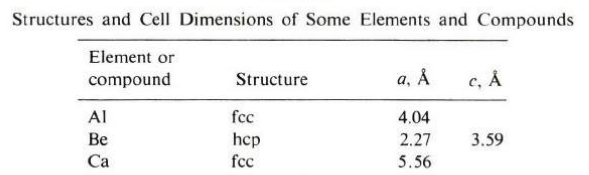
\includegraphics[width=0.7\linewidth]{Graphics/Chapter1/StructuresAndCellDimension_Table1_2_Omar}
	\caption{}
	\label{}
\end{figure}


\textbf{Unit Cell}
\begin{figure}[H]
	\centering
	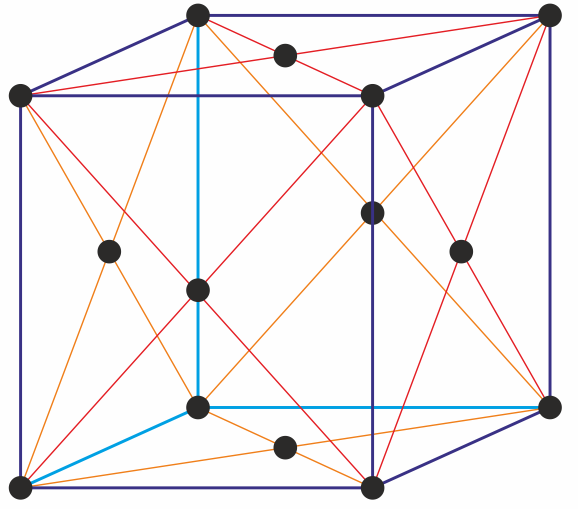
\includegraphics[width=0.4\linewidth]{Graphics/Chapter1/face-centered_cubic_lattice.png}
	\caption{}
	\label{}
\end{figure}

\textbf{Primitive Vectors}

The three primitive vectors are

$$\vec{u} = \frac{a}{2} \left(\begin{matrix}1\\1\\0\\\end{matrix}\right) \qquad
  \vec{v} = \frac{a}{2} \left(\begin{matrix}0\\1\\1\\\end{matrix}\right) \qquad
  \vec{w} = \frac{a}{2} \left(\begin{matrix}1\\0\\1\\\end{matrix}\right)$$

The volume can be calculated with the following formula

$$V_{PC} = \vert (\vec{u} \times \vec{v})  \cdot \vec{w} \vert$$

which equals (with $a = 5.56 \, \mathring{A}$)

$$V_{PC} = \frac{a^3}{4} = 4.297 \cdot 10^{-30} \,m^3 = 4.297 \cdot 10^{-24} \,cm^3$$
\textbf{Packaging Factor}

The Packaging Factor can be calculated as the ratio between the
volume of the atoms in the unit cell to the volume of the unit cell.

The volume of the unit cell can be calculated as:

$$V_{UC} = a^3$$


The unit cell containts 4 whole atoms 

The relationship between the parameter $a$ and the radius of the Radius of the atomic sphere is given as:
$$r = \frac{\sqrt{2}}{4} a $$

$$APF = \frac{\pi}{3 \cdot \sqrt{2}} \approx 74\%$$


\textbf{Density}

The atomic mass of calcium us given as:
$$M_{Ca} = 40.078 \frac{g}{mol}$$


$$\rho = \frac{4}{N_A} \cdot \frac{M_{Ca}}{V_{UC}} = 1.55 \frac{g}{cm^3}$$


\textbf{Planes}

In the following the planes $P1: \, (0\overline{3}2)$ and $P2: \,(\overline{1}21)$ are drawn inside the unit cell.
The Miller-Indices of the planes corresbond to the following plane equations:
$$P1: \quad -\frac{1}{3} y + \frac{1}{2} z = 1$$
$$P2: \quad -x +\frac{1}{2} y + z = 1$$

With respect of the fact that all parallel planes have the same Miller-Indices the planes which were drawn are:
$$P1: \quad z = \frac{2/}{3}y$$
$$P2: \quad z = x + -\frac{1}{2}y$$

\begin{figure}[H]
	\centering
	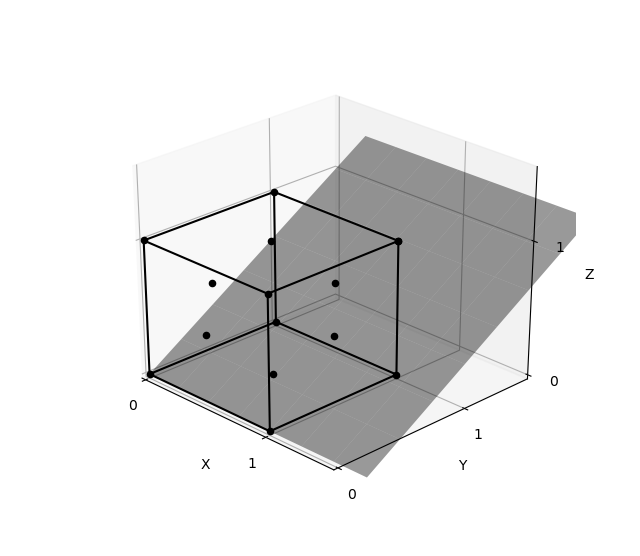
\includegraphics[width=0.6\linewidth]{Graphics/Chapter1/PLANE032}
	\caption{$(0\overline{3}2)$-Plane in an FCC lattice}
	\label{}
\end{figure}


\begin{figure}[H]
	\centering
	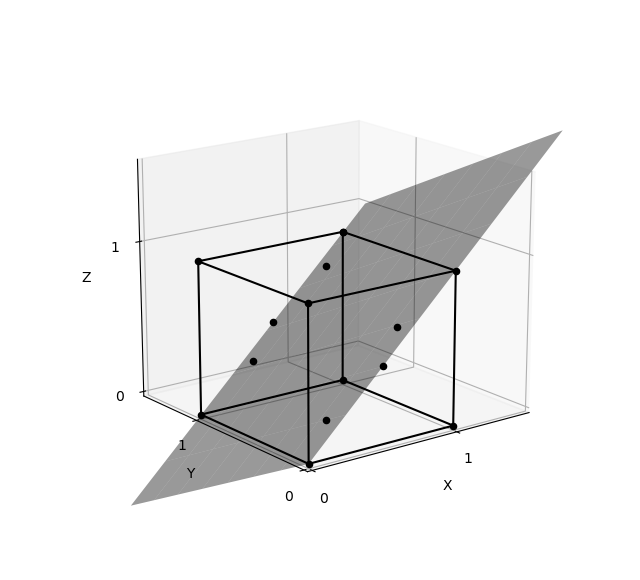
\includegraphics[width=0.6\linewidth]{Graphics/Chapter1/PLANE121}
	\caption{$(\overline{1}21)$-Plane in an FCC lattice}
	\label{}
\end{figure}


\textbf{Linear Density [110]}

$$\lambda = \frac{2 \cdot m_{Ca}}{\sqrt{2}a}$$
